% Options for packages loaded elsewhere
\PassOptionsToPackage{unicode}{hyperref}
\PassOptionsToPackage{hyphens}{url}
%
\documentclass[
]{book}
\usepackage{amsmath,amssymb}
\usepackage{iftex}
\ifPDFTeX
  \usepackage[T1]{fontenc}
  \usepackage[utf8]{inputenc}
  \usepackage{textcomp} % provide euro and other symbols
\else % if luatex or xetex
  \usepackage{unicode-math} % this also loads fontspec
  \defaultfontfeatures{Scale=MatchLowercase}
  \defaultfontfeatures[\rmfamily]{Ligatures=TeX,Scale=1}
\fi
\usepackage{lmodern}
\ifPDFTeX\else
  % xetex/luatex font selection
\fi
% Use upquote if available, for straight quotes in verbatim environments
\IfFileExists{upquote.sty}{\usepackage{upquote}}{}
\IfFileExists{microtype.sty}{% use microtype if available
  \usepackage[]{microtype}
  \UseMicrotypeSet[protrusion]{basicmath} % disable protrusion for tt fonts
}{}
\makeatletter
\@ifundefined{KOMAClassName}{% if non-KOMA class
  \IfFileExists{parskip.sty}{%
    \usepackage{parskip}
  }{% else
    \setlength{\parindent}{0pt}
    \setlength{\parskip}{6pt plus 2pt minus 1pt}}
}{% if KOMA class
  \KOMAoptions{parskip=half}}
\makeatother
\usepackage{xcolor}
\usepackage{color}
\usepackage{fancyvrb}
\newcommand{\VerbBar}{|}
\newcommand{\VERB}{\Verb[commandchars=\\\{\}]}
\DefineVerbatimEnvironment{Highlighting}{Verbatim}{commandchars=\\\{\}}
% Add ',fontsize=\small' for more characters per line
\usepackage{framed}
\definecolor{shadecolor}{RGB}{248,248,248}
\newenvironment{Shaded}{\begin{snugshade}}{\end{snugshade}}
\newcommand{\AlertTok}[1]{\textcolor[rgb]{0.94,0.16,0.16}{#1}}
\newcommand{\AnnotationTok}[1]{\textcolor[rgb]{0.56,0.35,0.01}{\textbf{\textit{#1}}}}
\newcommand{\AttributeTok}[1]{\textcolor[rgb]{0.13,0.29,0.53}{#1}}
\newcommand{\BaseNTok}[1]{\textcolor[rgb]{0.00,0.00,0.81}{#1}}
\newcommand{\BuiltInTok}[1]{#1}
\newcommand{\CharTok}[1]{\textcolor[rgb]{0.31,0.60,0.02}{#1}}
\newcommand{\CommentTok}[1]{\textcolor[rgb]{0.56,0.35,0.01}{\textit{#1}}}
\newcommand{\CommentVarTok}[1]{\textcolor[rgb]{0.56,0.35,0.01}{\textbf{\textit{#1}}}}
\newcommand{\ConstantTok}[1]{\textcolor[rgb]{0.56,0.35,0.01}{#1}}
\newcommand{\ControlFlowTok}[1]{\textcolor[rgb]{0.13,0.29,0.53}{\textbf{#1}}}
\newcommand{\DataTypeTok}[1]{\textcolor[rgb]{0.13,0.29,0.53}{#1}}
\newcommand{\DecValTok}[1]{\textcolor[rgb]{0.00,0.00,0.81}{#1}}
\newcommand{\DocumentationTok}[1]{\textcolor[rgb]{0.56,0.35,0.01}{\textbf{\textit{#1}}}}
\newcommand{\ErrorTok}[1]{\textcolor[rgb]{0.64,0.00,0.00}{\textbf{#1}}}
\newcommand{\ExtensionTok}[1]{#1}
\newcommand{\FloatTok}[1]{\textcolor[rgb]{0.00,0.00,0.81}{#1}}
\newcommand{\FunctionTok}[1]{\textcolor[rgb]{0.13,0.29,0.53}{\textbf{#1}}}
\newcommand{\ImportTok}[1]{#1}
\newcommand{\InformationTok}[1]{\textcolor[rgb]{0.56,0.35,0.01}{\textbf{\textit{#1}}}}
\newcommand{\KeywordTok}[1]{\textcolor[rgb]{0.13,0.29,0.53}{\textbf{#1}}}
\newcommand{\NormalTok}[1]{#1}
\newcommand{\OperatorTok}[1]{\textcolor[rgb]{0.81,0.36,0.00}{\textbf{#1}}}
\newcommand{\OtherTok}[1]{\textcolor[rgb]{0.56,0.35,0.01}{#1}}
\newcommand{\PreprocessorTok}[1]{\textcolor[rgb]{0.56,0.35,0.01}{\textit{#1}}}
\newcommand{\RegionMarkerTok}[1]{#1}
\newcommand{\SpecialCharTok}[1]{\textcolor[rgb]{0.81,0.36,0.00}{\textbf{#1}}}
\newcommand{\SpecialStringTok}[1]{\textcolor[rgb]{0.31,0.60,0.02}{#1}}
\newcommand{\StringTok}[1]{\textcolor[rgb]{0.31,0.60,0.02}{#1}}
\newcommand{\VariableTok}[1]{\textcolor[rgb]{0.00,0.00,0.00}{#1}}
\newcommand{\VerbatimStringTok}[1]{\textcolor[rgb]{0.31,0.60,0.02}{#1}}
\newcommand{\WarningTok}[1]{\textcolor[rgb]{0.56,0.35,0.01}{\textbf{\textit{#1}}}}
\usepackage{longtable,booktabs,array}
\usepackage{calc} % for calculating minipage widths
% Correct order of tables after \paragraph or \subparagraph
\usepackage{etoolbox}
\makeatletter
\patchcmd\longtable{\par}{\if@noskipsec\mbox{}\fi\par}{}{}
\makeatother
% Allow footnotes in longtable head/foot
\IfFileExists{footnotehyper.sty}{\usepackage{footnotehyper}}{\usepackage{footnote}}
\makesavenoteenv{longtable}
\usepackage{graphicx}
\makeatletter
\def\maxwidth{\ifdim\Gin@nat@width>\linewidth\linewidth\else\Gin@nat@width\fi}
\def\maxheight{\ifdim\Gin@nat@height>\textheight\textheight\else\Gin@nat@height\fi}
\makeatother
% Scale images if necessary, so that they will not overflow the page
% margins by default, and it is still possible to overwrite the defaults
% using explicit options in \includegraphics[width, height, ...]{}
\setkeys{Gin}{width=\maxwidth,height=\maxheight,keepaspectratio}
% Set default figure placement to htbp
\makeatletter
\def\fps@figure{htbp}
\makeatother
\setlength{\emergencystretch}{3em} % prevent overfull lines
\providecommand{\tightlist}{%
  \setlength{\itemsep}{0pt}\setlength{\parskip}{0pt}}
\setcounter{secnumdepth}{5}
\usepackage{booktabs}
\usepackage{amsthm}
\makeatletter
\def\thm@space@setup{%
  \thm@preskip=8pt plus 2pt minus 4pt
  \thm@postskip=\thm@preskip
}
\makeatother
\ifLuaTeX
  \usepackage{selnolig}  % disable illegal ligatures
\fi
\usepackage[]{natbib}
\bibliographystyle{apalike}
\IfFileExists{bookmark.sty}{\usepackage{bookmark}}{\usepackage{hyperref}}
\IfFileExists{xurl.sty}{\usepackage{xurl}}{} % add URL line breaks if available
\urlstyle{same}
\hypersetup{
  pdftitle={Introduction to R},
  pdfauthor={Ryan Donovan},
  hidelinks,
  pdfcreator={LaTeX via pandoc}}

\title{Introduction to R}
\author{Ryan Donovan}
\date{2024-01-19}

\begin{document}
\maketitle

{
\setcounter{tocdepth}{1}
\tableofcontents
}
\hypertarget{introduction}{%
\chapter{Introduction}\label{introduction}}

This set of workshops describes how to use R to import, clean, and process psychological data. All materials, data, and information in these workshops are used for educational purposes only. This document should only be shared within the University of Galway's School of Psychology, and is not intended for widespread dissemination. The workshop's e-book is very much in its draft stages and will be updated and fine-tuned in the future. Several materials are adapted from several online resources on teaching R.

\hypertarget{who-is-this-resource-for}{%
\section{Who is this resource for?}\label{who-is-this-resource-for}}

These workshops are designed to help people who come from a Psychology or social science background learn the necessary programming skills to use R effectively in their research. These workshops are designed to help people who have no programming experience whatsoever to learn the necessary programming skills and ideas that you will need to conduct typically statistical techniques in Psychology (e.g., Power Analyses, Correlation, ANOVA, Regression, Mediation, Moderation).

These workshops are \textbf{\emph{not}} for people interested in learning about statistical theory or the who, what, where's of any of the aforementioned statistical techniques. I want these workshops to focus entirely on how to do statistical analyses in R - I assume you know the rest or know how to access that information.

\hypertarget{should-i-learn-r}{%
\section{Should I learn R?}\label{should-i-learn-r}}

There are a lot of reasons to learn R.

Psychological research is increasingly moving towards open-science practices. One of the key principles of open-science is that all aspects of data handling - including data wrangling, pre-processing, processing, and output generation are openly accessible. This is not only an abstract want or desire, several top-tier journals require that you submit R scripts along with any manuscripts. If you don't know how to use R (or at least no one in your lab does), then this will put you at an disadvantage.

R enables you to import, clean, analysis and publish manuscripts from R itself. You do not have to switch between SPSS, Excel, and Word or any other software. You can conduct your statistical analysis directly in R and have that ``uploaded'' directly to your manuscript. In the long run, this will save you so much time and energy.

R is capable of more than statistical analysis. You can create websites, documents, and books in R. This workshop textbook was developed in R! While these initial workshops will not be discussing how to do this (although it is something that I would like to do in the future), I wanted to mention it as an example how powerful R can be.

\hypertarget{what-will-i-learn-to-do-in-r}{%
\section{What will I learn to do in R?}\label{what-will-i-learn-to-do-in-r}}

The following workshops will teach you on how to conduct statistical analysis in R.

R is a statistical programming language that enables you to wrangle, process, and analyse data. By the end of these workshops you should be able to import a data file into R, do some processing and cleaning, compute descriptive and inferential statistics, generate nice visualizations, and output your results.

The learning objectives of this course are:

\begin{itemize}
\tightlist
\item
  Learn how to import and create data sets in R.
\item
  Learn and apply basic programming concepts such as data types, functions, and loops.
\item
  Learn key techniques for data cleaning in R to enable statistical analysis
\item
  Learn how to create APA-standard graphs in R
\item
  Learn how to deal with errors or bugs with R code
\item
  Learn how to export data.
\end{itemize}

\hypertarget{what-will-i-not-learn-to-do-in-r}{%
\section{What will I not learn to do in R?}\label{what-will-i-not-learn-to-do-in-r}}

This is not an exhaustive introduction to R. Similar to human languages, programming languages like R are vast and will take years to master. After this course, you will still be considered a ``newbie'' in R. But the material covered here will at least provide you a solid foundation in R, enabling you to go ahead and pick up further skills if required as you go on.

This course will teach you data cleaning and wrangling skills that you will enable you to wrangle and clean a lot of data collected on Gorilla or Qualtrics. But you will not be able to easily handle all data cleaning problems you are likely to find out in the ``wild'' world of messy data. Such data sets can be uniquely messy, and even experience R programmers will need to bash their head against the wall a few times to figure out a way to clean that data set entirely in R. If you have a particularly messy data set, you might still need to use other programs (e.g., Excel) to clean it up first before importing it to R.

Similarly, do not expect to be fluent in the concepts you learn here after these workshops. It will take practice to become fluent. You might need to refer to these materials or look up help repeatedly when using R on real-life data sets. That's normal.

This workshop is heavily focused on the tidyverse approach to R. The tidyverse is a particular philosophical approach on how to use R (more on that later). The other approach would be to use base R. This can incite violent debates in R communities on which approach is better. We will focus mainly on tidyverse and use some base R.

This workshop does not teach you on how to use R Markdown. R Markdown is a package in R that enables you to write reproducible and dynamic reports with R that can be converted into word documents, PDFS, websites, power point presentations, books, and much more. That will be covered in the intermediate workshop program.

\hypertarget{where-and-when-will-the-workshops-take-place}{%
\section{Where and when will the workshops take place?}\label{where-and-when-will-the-workshops-take-place}}

The sessions will take place in \textbf{\emph{AMB-G035}} (Psychology PC Suite). The schedule for the sessions is as follows:

\begin{itemize}
\tightlist
\item
  Feb 7th: Introduction to R and RStudio
\item
  Feb 14th: Basic Programming (Part I)
\item
  Feb 21st: Basic Programming (Part II)
\item
  Feb 28th: Data Cleaning in R (Part I)
\item
  March 6th: Data Cleaning in R (Part II)
\item
  March 13th: Data Visualization
\item
  March 20th: Running Inferential Statistical Tests in R (Part I)
\item
  March 27th: Running Inferential Statistical Tests in R (Part II)
\end{itemize}

Each session is on a Wednesday and will run between 11:00 - 13:00.

\hypertarget{are-they-any-prerequisites-for-taking-this-course}{%
\section{Are they any prerequisites for taking this course?}\label{are-they-any-prerequisites-for-taking-this-course}}

None at all. This course is beginners friendly. You also do not need to purchase anything (e.g., textbook, or software).

\hypertarget{do-i-need-to-bring-a-laptop-to-the-class}{%
\section{Do I need to bring a laptop to the class?}\label{do-i-need-to-bring-a-laptop-to-the-class}}

If you have a laptop that you work on, I strongly encourage you to bring it. That way we can get R and RStudio installed onto your laptop and you'll be able to run R outside of the classroom.

If you work with a desktop, don't worry. The lab space will have computers that you can sign-in and work on and use R.

\hypertarget{rstudio}{%
\chapter{Getting Started with R and RStudio}\label{rstudio}}

This workshop introduces the programming language R and the RStudio application. Today, we will download both R and RStudio, set up our RStudio environment, and write and run our first piece of R Code. This will set us up for the rest of the workshops.

\hypertarget{what-actually-is-r}{%
\section{What actually is R?}\label{what-actually-is-r}}

R is a statistical programming language that enables us to directly ask our computer to carry out tasks. Typically, when we use our computers, we do not speak to it directly; instead we interact with ``translators'' (i.e., applications like SPSS), via button-click interfaces, to speak to our computer on our behalf. Such interfaces record and translate our instructions to our computers, who then carry out the instructions and return the results to the application, which then translates those results back to us.

Applications like SPSS are convenient. They usually have a user-friendly button-click based interface and take away the heavy lifting of communicating with our computer. This makes them significantly easier to learn in the short term compared to programming languages.

However, these apps also limit what we can do. For example, base SPSS is functional when it comes to creating visualizations, but it is difficult make major changes to your graph (e.g., making it interactive). If we want to create such visualizations, we will likely need to look elsewhere for it. Similarly, we might also be financially limited in our ability to use such apps, as proprietary software like SPSS is not cheap (\href{https://www.ibm.com/products/spss-statistics/pricing}{it can cost between \$3830 - 25200 for a single licence depending on the version})!

In contrast, R is a free, open-source statistical programming language that enables us to conduct comprehensive statistical analysis and create highly elegant visualizations. By learning R we can cut out the middle man.

\begin{figure}
\centering
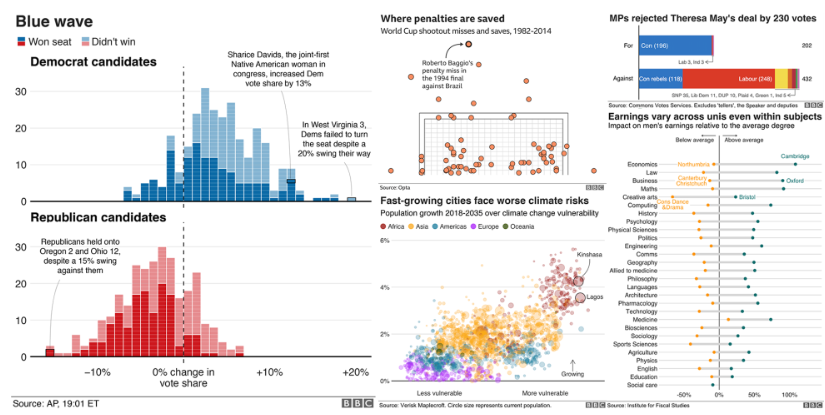
\includegraphics{img/01-bbc.png}
\caption{\label{fig:unnamed-chunk-1}BBC graphs created in R.}
\end{figure}

But why should we learn R and not a different programming language? In contrast to other programming languages (Python, JavaScript, C), R was developed by statisticians. Consequently, R contains an extensive vocabulary to enable us to carry out sophisticated and precise statistical analysis. I have used R and Python to conduct statistical analysis and anytime I wanted to use a less frequently used statistical test, there was significantly more support and information on how to conduct that analysis in R than in Python. For such reasons, R is typically used among statisticians, social scientists, data miners, and bioinformaticians - and will be used in this course\footnote{There are always tradeoffs in selecting a language. Many programming concepts are easier to grasp in Python than in R. Similarly, there is a lot of resources available for conducting machine-learning analysis in Python.

  But if you are goal is conduct data cleaning, analysis, visualization, and reporting, then R is a excellent choice. The good thing is that once you achieve a certain level of competency in one programming language, you will find it significantly easier to pick up a following one.}.

\hypertarget{downloading-r}{%
\section{Downloading R}\label{downloading-r}}

Please follow the following instructions to download R on either Windows or Mac.

\hypertarget{downloading-r-on-windows}{%
\subsection{Downloading R on Windows}\label{downloading-r-on-windows}}

\begin{enumerate}
\def\labelenumi{\arabic{enumi}.}
\tightlist
\item
  Go to the website: \url{https://cran.r-project.org/}
\item
  Under the heading \emph{Download and Install R,} click \emph{Download R for Windows} 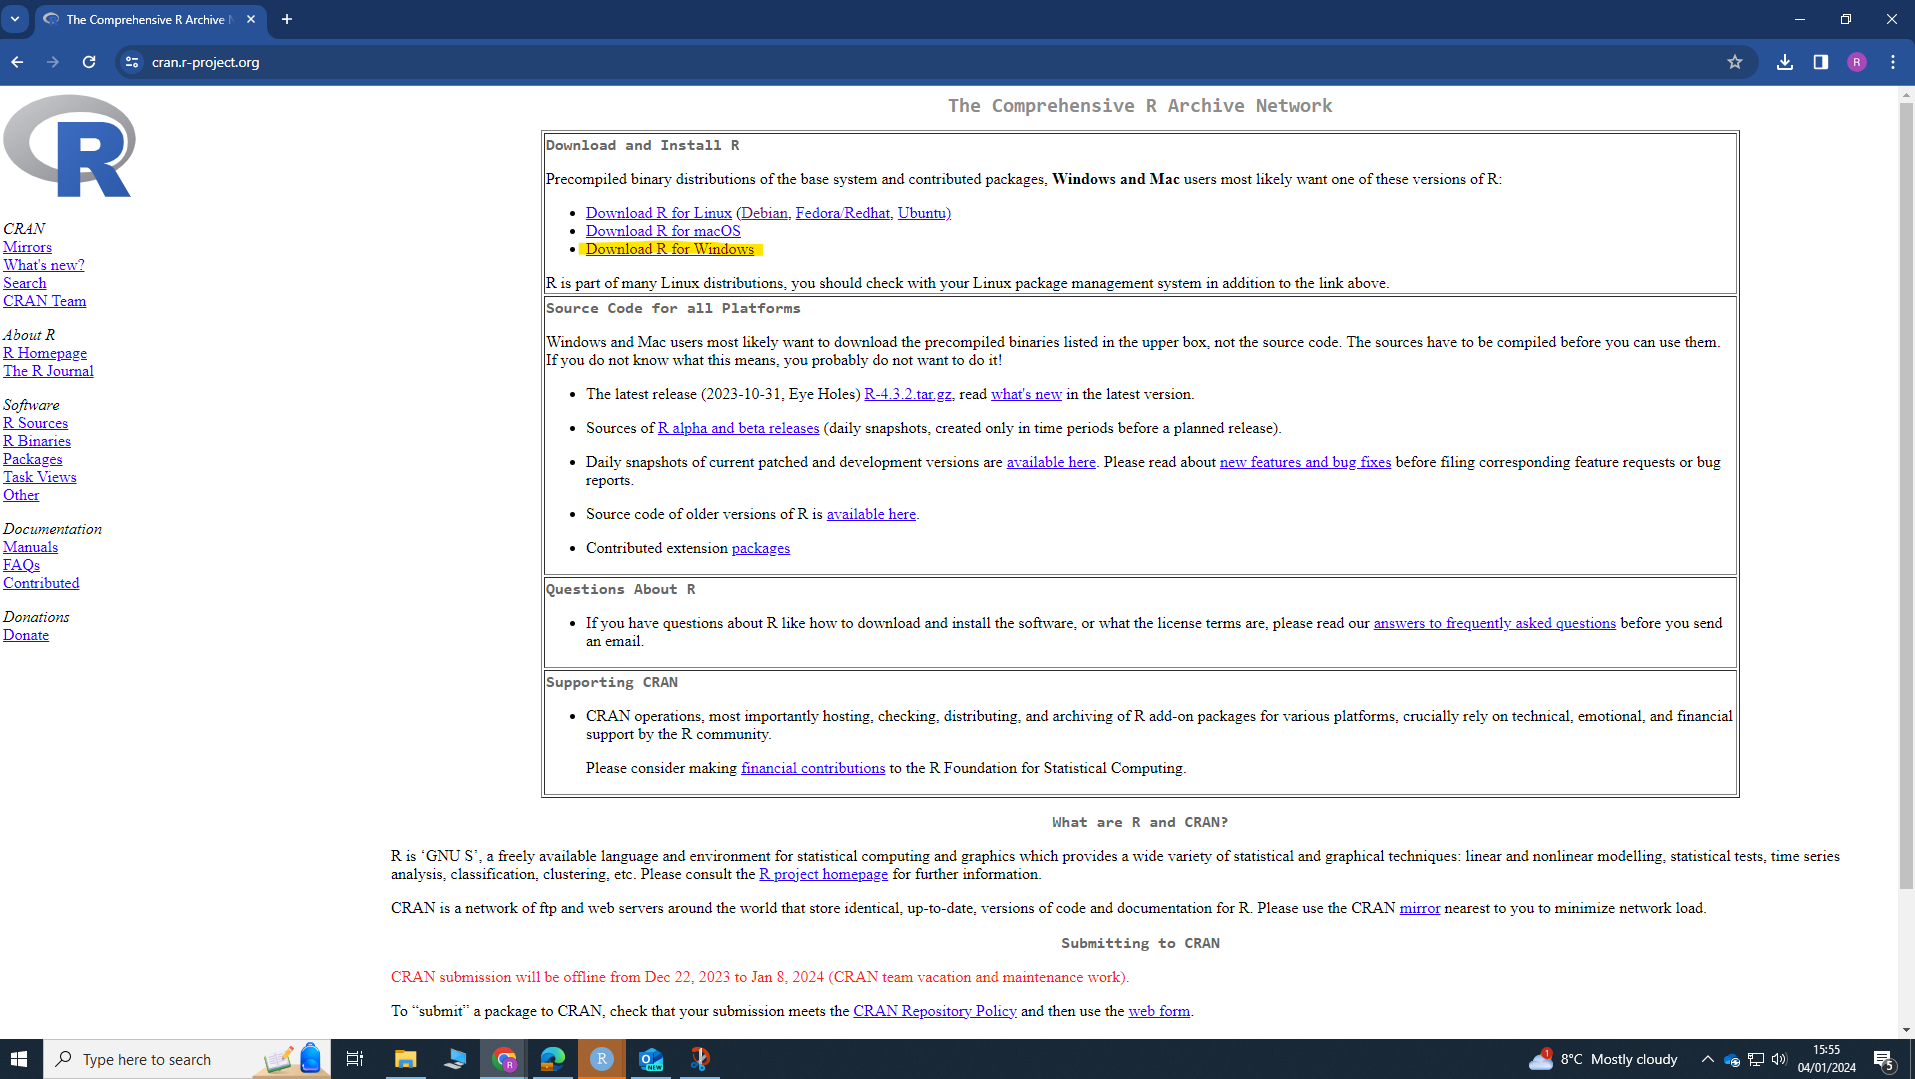
\includegraphics[width=29.20833in,height=\textheight]{img/01-cran.png}
\item
  Click the hyperlink \textbf{\emph{base}} or \textbf{\emph{install R for the first Time}}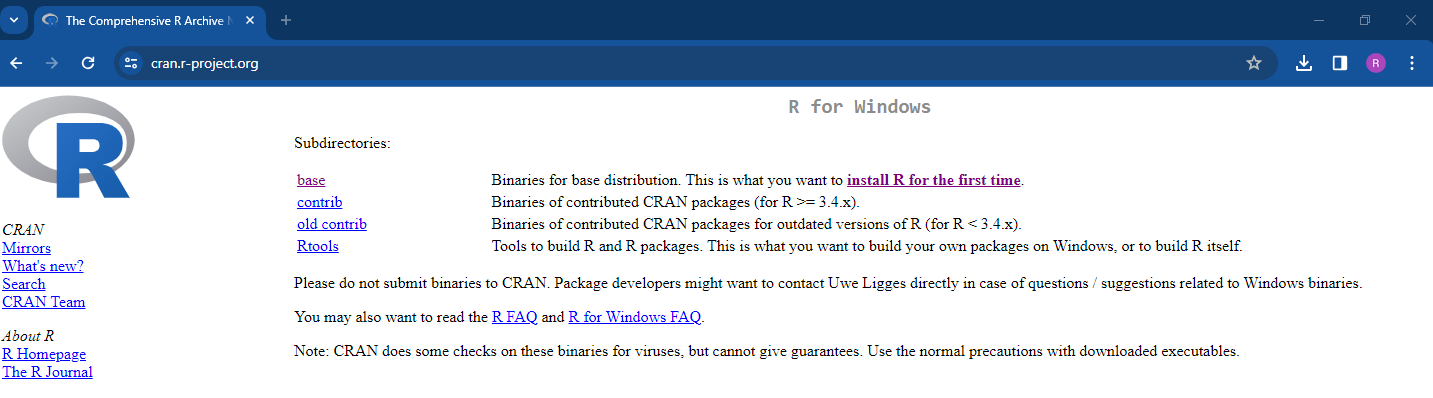
\includegraphics{img/01-base.png}
\item
  Click Download R-4.3.2 for Windows (depending on the date you accessed this, the version of R might have been been updated. That's okay, you can download newer versions). Let the file download. 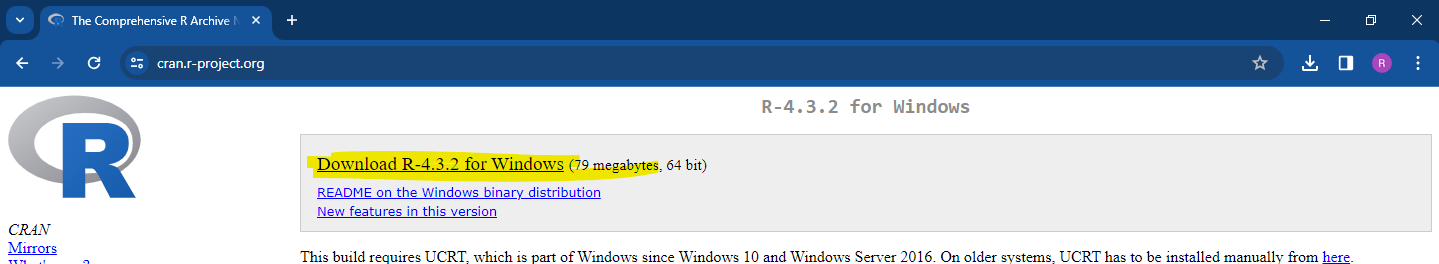
\includegraphics{img/01-download.png}
\item
  Once the file has been downloaded, open it, and click ``Yes'' if you are asked to allow this app to make changes to your device. Then choose English as your setup language. The file name should be something like ``R-4.3.2.-win''. The numbers will differ depending on the specific version that was downloaded.
\item
  Agree to the terms and conditions and select a place to install R. It is perfectly fine to go with the default option.
\end{enumerate}

\hypertarget{downloading-r-on-mac}{%
\subsection{Downloading R on Mac}\label{downloading-r-on-mac}}

The instructions are largely the same for Windows. Please see this guide for more information \url{https://teacherscollege.screenstepslive.com/a/1135059-install-r-and-r-studio-for-mac}

\hypertarget{install-and-open-r-studio}{%
\section{Install and Open R Studio}\label{install-and-open-r-studio}}

Once R is installed, we will install RStudio.

RStudio is a front-end program that makes it it much more user-friendly to use R without sacrificing our ability to code in R. R Studio will enable us to write and save R code, generate plots, manage our files, and do other useful things. RStudio relationship to R is similar to the relationship between a basic text editor and Microsoft Word. We could write a paper in a text editor, but it is much quicker and more efficient to use Word.

\begin{enumerate}
\def\labelenumi{\arabic{enumi}.}
\tightlist
\item
  \textbf{NB:} Make sure that R is installed \textbf{\emph{before}} trying to install R Studio.
\item
  Go to the RStudio website: \url{https://posit.co/download/rstudio-desktop/}
\item
  The website should automatically detect your operating system. Click the \textbf{\emph{Download RStudio Desktop}} button. 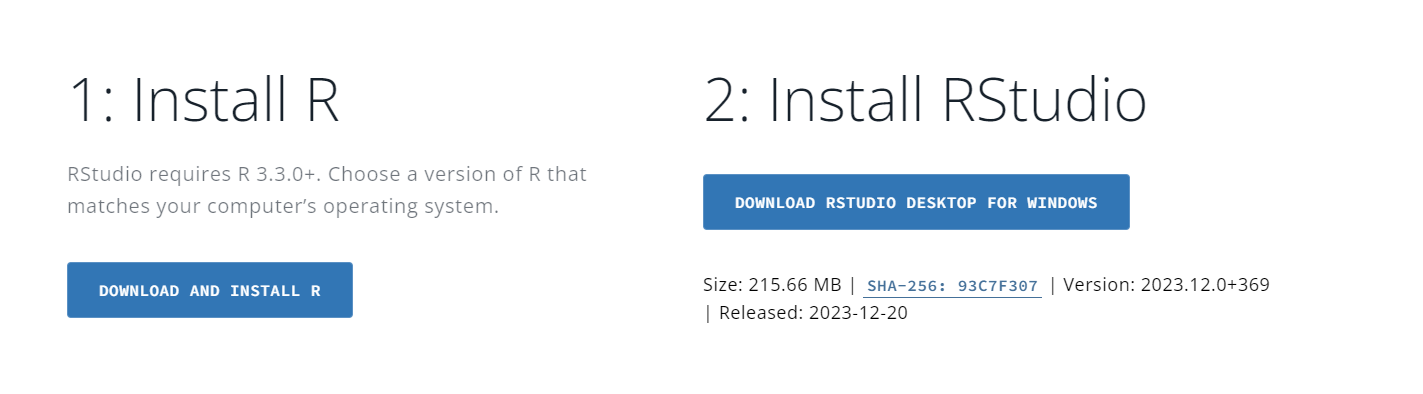
\includegraphics[width=7.1875in,height=\textheight]{img/01-rstudiodownload.png}
\end{enumerate}

Once the file is downloaded, open it and allow it to make changes to your device. Then follow the instructions to download the program. I recommend going with all default options here.

After downloading both R and RStudio, open RStudio on your computer. You do not have to open R as RStudio will work with R (if everything is working correctly).

When you first open RStudio, you will see three panes or ``windows'' in R Studio: ``Console'' (left) ``Environment'' (top right), and ``Files'' (bottom right).

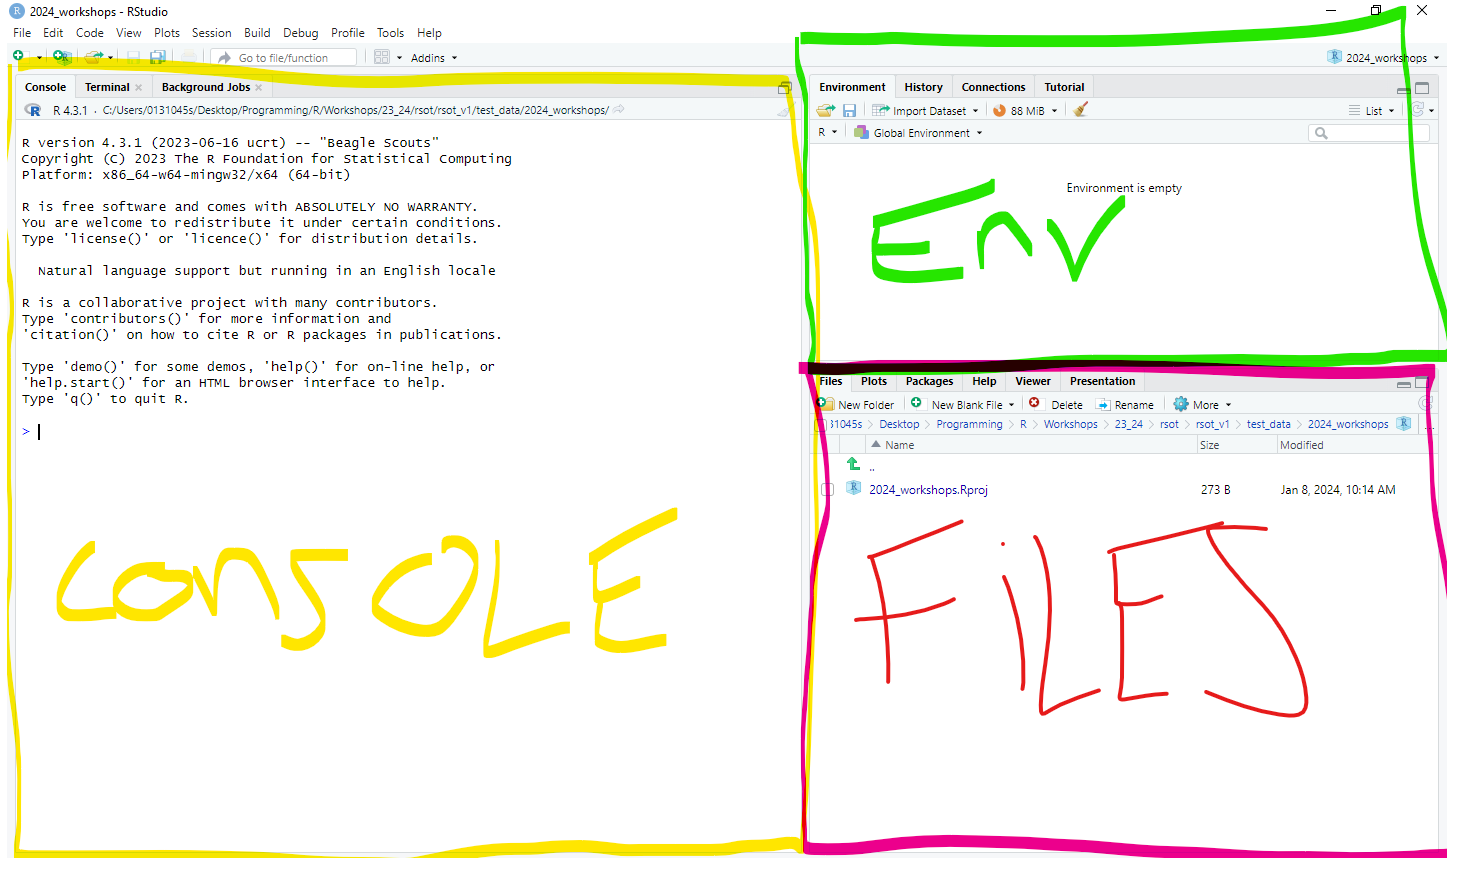
\includegraphics{img/rstudio_first.png}

\hypertarget{creating-an-r-project}{%
\section{Creating an R Project}\label{creating-an-r-project}}

The first thing we will do in RStudio is create a \emph{R Project}. R Projects are environments that will group together input files (e.g., data sets), analyses on those files (e.g., code), and any outputs (e.g., results or plots). Creating an R Project will set up a new directory (folder) on your computer. Any time you open that project, you are telling R to work within this particular directory.

\textbf{\emph{Activity}}

Let's create an R Project that we will use during these workshops.

\begin{enumerate}
\def\labelenumi{\arabic{enumi}.}
\item
  Click ``File'' in the top left hand corner of RStudio-\textgreater{} then click new ``New Project''
\item
  The ``New Project Wizard'' screen will pop up. Click ``New Directory'' -\textgreater{} ``New Project''
\item
  In the ``Create New Project'' screen, there are four options.
\end{enumerate}

\textbf{Option 1}: The ``Directory name'' options sets the name of the project and associated folder.

\begin{itemize}
\item
  You can set this to whatever you want. \textbf{\emph{Just don't set it to ``R'',}} as this can create problems down the line.
\item
  I \textbf{\emph{recommend}} that you set the same directory name as me - \textbf{\emph{introR\_2024}}
\end{itemize}

\textbf{Option 2}: The ``Create project as sub-directory of'' option selects a place to store this project on your computer.

\begin{itemize}
\item
  You can save this anywhere else you like (e.g., your Desktop). Just make sure to save somewhere you can find and somewhere that will not change location (e.g., if you save folders to your desktop, but then tend to move them elsewhere once it gets cluttered, then do not save it to your desktop).
\item
  My recommendation would be to create a folder called ``R\_Programming'' on your desktop. And then save your project in this folder.
\item
  Regardless of where you save your project, copy the location and paste it somewhere you can check (e.g., into a text file)
\end{itemize}

\textbf{Option 3}: The ``Use renv with this project'' option enables you to create a virtual environment for this project that will be separate to other R projects. Don't worry for now about what that means, it will be explained later on.

\begin{itemize}
\tightlist
\item
  Tick this option.
\end{itemize}

\textbf{Option 4:} The ``Open in new session'' just opens a new window on RStudio for this project.

\begin{itemize}
\tightlist
\item
  Tick this option.
\end{itemize}

You can see my example below. Once you're happy with your input for each option, click ``Create Project'' This will open up the project introR\_2024.

\begin{figure}
\centering
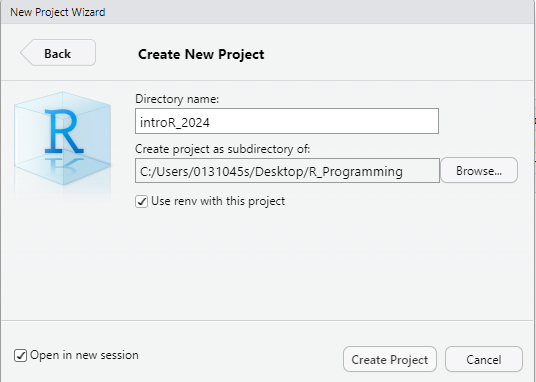
\includegraphics{img/01-newproject.png}
\caption{\label{fig:unnamed-chunk-2}New Project Set Up}
\end{figure}

\hypertarget{navigating-rstudio}{%
\subsection{Navigating RStudio}\label{navigating-rstudio}}

In our new project, introR\_2024, we are going to open the ``Source'' pane, which we will often use for writing code, and viewing datasets.

There are a variety of ways to open the Source pane.

\textbf{Button approach}: Click the ``File'' tab in the top-left hand corner (not the File pane) -\textgreater{} Click ``New File'' -\textgreater{} ``R Script''

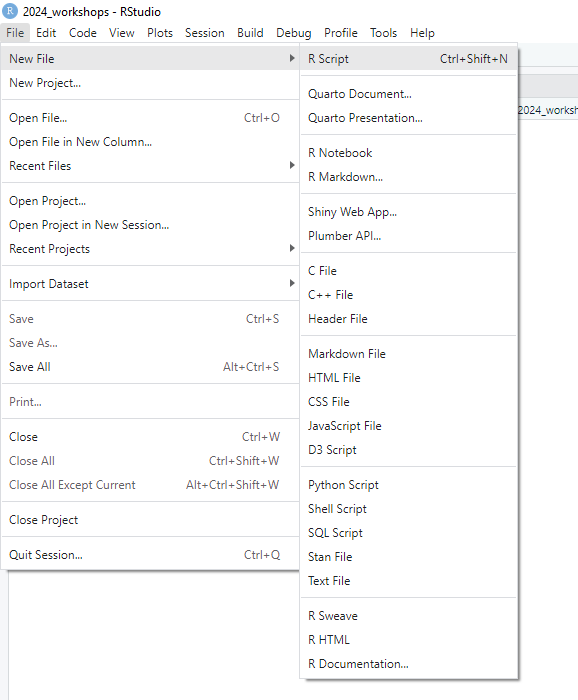
\includegraphics{img/rstudio_create_file.png}

\textbf{\emph{Button Shortcut}}: directly underneath the \emph{File} tab, there is an icon of a white sheet with a green and white addition symbol. You can click that too.

\textbf{Keyboard Shortcut:} You can press ``Ctrl'' + ``Shift'' and ``N'' on Windows. Or ``Cmd'' + ``Shift'' + ``N'' on Mac.

Now you should see your four panes: Source, Console, Environment, and Files.

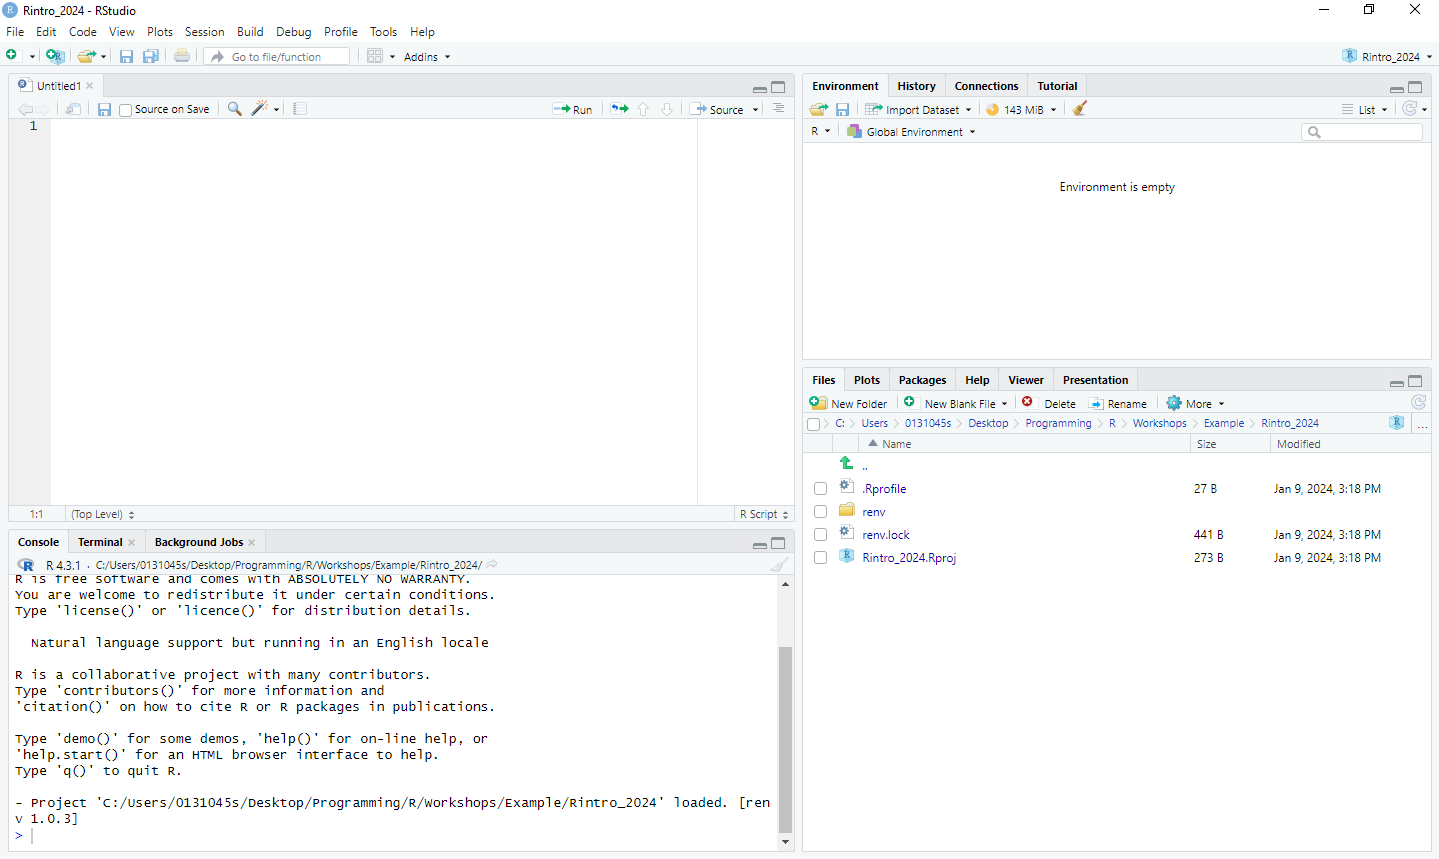
\includegraphics{img/01-four-panes.png}

\hypertarget{the-rstudio-workspace}{%
\subsubsection{The RStudio Workspace}\label{the-rstudio-workspace}}

Now that we have each pane opened, let's briefly describe what each pane is for.

\begin{itemize}
\item
  The \textbf{\emph{Source Pane}} is where you will write R scripts. R scripts enable you to write, save, and run R code in a structured format. For example, you might have an R script titled ``Descriptive'' which contains the code you need to compute descriptive statistics on your data set. Similarly, you might have another R script titled ``Regression'' that contains the code for computing your regression analyses in R.
\item
  The \textbf{\emph{Console Pane}} is where you can write R code or enter commands into R. The console is also where you can find several outputs from your R scripts. For example, if you create a script for running a t-test in R, then the results can be found in the Console Pane. You will also find any error or warning messages about any code that you run (e.g., if you make a mistake in your R code) highlighted in the console. In short, the console is where R is actually running.
\item
  The \textbf{\emph{Environment Pane}} is where you will find information on any data sets and variables that you import or create in R within a bespoke R project. The ``History'' tab will contain a history of any R code that you run during the project. This pane is really useful for getting a bird-eye's view of a project (which can be really useful if you are returning to a project after a long period of time or you are looking at someone's else code).
\item
  The \textbf{\emph{Files Pane}} is where you find your R project files (in the Files tab), the output of any plots that you create (Plots tab), the status of any downloaded packages (Packages tab), and information and helpful information about R functions and packages (Help).
\end{itemize}

Each pane will be used extensively during these workshops.

\hypertarget{checking-our-working-directory}{%
\subsection{Checking our Working Directory}\label{checking-our-working-directory}}

Everytime you open up a project or file in RStudio, it is good practice to check the working directory. The working directory is the environment on our computer that R is currently operating in.

You want the working directory to be in the same location as your R project. That way any files you import into RStudio or any files you export (datasets, results, graphs) can easily be found in your R project folder. A lot of problems can be avoided in R by making sure that you check the working directory.

To check the working directory, type the following into the console pane

\begin{Shaded}
\begin{Highlighting}[]
\FunctionTok{getwd}\NormalTok{()}
\end{Highlighting}
\end{Shaded}

\begin{verbatim}
## [1] "C:/Users/0131045s/Desktop/Programming/R/Workshops/rintro"
\end{verbatim}

What you get in return is the current working directory R is working in. Your working directory will not be the same as mine, that's perfectly normal. Just check to make sure that is in the same location you specified when you created your project (\textbf{Option 2}).

\hypertarget{setting-up-a-new-working-directory}{%
\subsection{Setting up a new Working Directory}\label{setting-up-a-new-working-directory}}

We are going to slightly change our working directory. In our R Project, we are going to create a folder for week1 of the workshop. Anything that we create in R will then be saved into this week1 folder.

\begin{itemize}
\tightlist
\item
  Click ``Session'' on your RStudio toolbar -\textgreater{} Set Working Directory -\textgreater{} Choose Directory
\end{itemize}

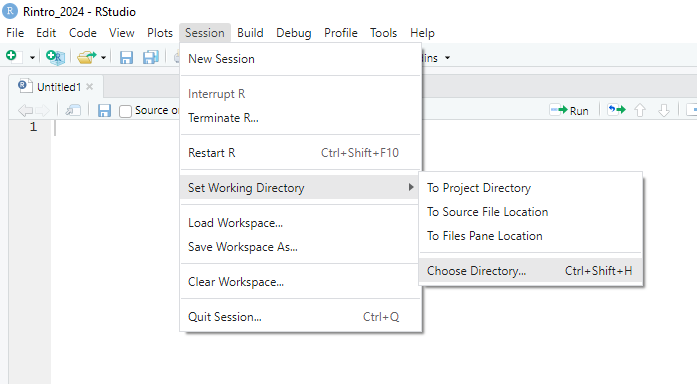
\includegraphics{img/01-wd.png}

\begin{itemize}
\item
  By default you should be in your R Project (e.g., Rintro\_2024).
\item
  Within this R Project, create a new folder and call it ``week1''
\item
  Click ``week1'' and then click Open
\end{itemize}

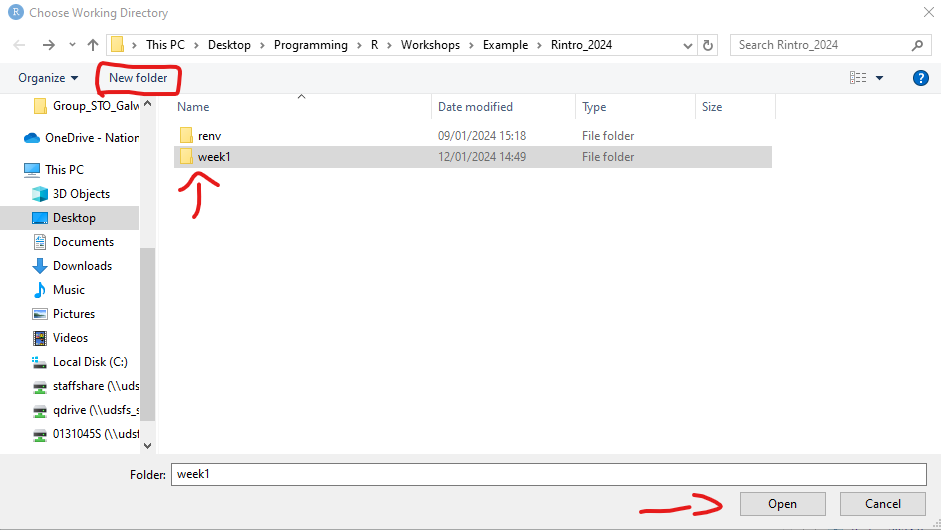
\includegraphics{img/01-new_wd.png}

You should see something like the following in your console

\begin{verbatim}
> setwd("C:/Users/0131045s/Desktop/Programming/R/Workshops/Example/Rintro_2024/week1")
\end{verbatim}

Check whether this is actually the location you want to store your files for this course. If it is, we are good to go. If not, then let me know.

\hypertarget{writing-our-first-r-code}{%
\section{Writing our first R Code}\label{writing-our-first-r-code}}

Let's write our first line of R code. In the \textbf{\emph{console}}, type in the each of the following instructions and press enter. Feel free to change the second line of code to add your own name.

\begin{Shaded}
\begin{Highlighting}[]
\FunctionTok{print}\NormalTok{(}\StringTok{"Hello World"}\NormalTok{)}
\end{Highlighting}
\end{Shaded}

\begin{verbatim}
## [1] "Hello World"
\end{verbatim}

\begin{Shaded}
\begin{Highlighting}[]
\FunctionTok{print}\NormalTok{(}\StringTok{"My name is Ryan and I am learning to code in R"}\NormalTok{)}
\end{Highlighting}
\end{Shaded}

\begin{verbatim}
## [1] "My name is Ryan and I am learning to code in R"
\end{verbatim}

Congratulations, you've written your first piece of code!

Let's describe what is going on here. We used a function called \texttt{print()} to print the words ``Hello World'' and ``My name is Ryan and I am learning to code in R'' in the console. Functions are equivalent to verbs in English language - they describe doing things. In this case, R sees the function print - then it looks inside the bracket to see what we want to print, and then it goes ahead and prints it. Pretty straightforward.

Functions are a very important programming concept, and there is a lot more going on under the hood than I have described so far - so we will be returning to functions repeatedly and filling you in with more information. But in essence functions are verbs that enable us to tell our computer to carry out specific actions on objects.

\hypertarget{console-vs-source-script}{%
\section{Console vs Source Script}\label{console-vs-source-script}}

You might have noticed that I asked you to write code in the console rather than in the source pane. It's worth discussing here what the differences are between the console and the script when it comes to writing code.

The console is like the immediate chat with R. It's where you can type and execute single lines of code instantly. Imagine it as a friendly conversation where you ask R to do something, and it responds right away. The console The console is fantastic for experimenting and getting instant feedback. It's your interactive playground, perfect for spontaneous interactions with R.

The console is also really useful for performing quick calculations, testing functions or pieces of code, and for running code that should run once and only once.

However, the console is cumbersome to use if we want to write code that is several lines long and/or when we want to structure or save our code. This is where R scripts come in.

R scripts are text files where we can write R code in a structured manner. Scripts enable us to structure our code (e.g., with headings and instructions), write several pieces of code, and save and rerun code easily. If you think of your console as a draft, then your script is for the code that you want to keep.

From now on, whenever we write code, we are going to be using R scripts by default. For the times we will write code in the console, I will let you know beforehand.

\hypertarget{lets-write-some-statistical-code}{%
\section{Let's write some statistical code}\label{lets-write-some-statistical-code}}

Okay we have talked a lot about R and RStudio. To finish off this session, let's write code that will take a data set, calculate some descriptive statistics, run an inferential test, generate a graph, and save our results. Don't worry if you do not understand any of the following code. Just follow along and type it yourself in the R script we opened up earlier (if it's not open, click ``File'' -\textgreater{} New File -\textgreater{} RScript)

When you download R, you will have automatic access to several functions (e.g., print) and data sets. One of these data sets are called sleep, which we are going to use right now. To learn more about the sleep data set, type \texttt{?sleep} into the console. You will find more information on the data sets in the Files pane, under the Help tab.

First let's have a look at the sleep data set by writing and running the following code.

\begin{Shaded}
\begin{Highlighting}[]
\FunctionTok{print}\NormalTok{(sleep) }
\end{Highlighting}
\end{Shaded}

\begin{verbatim}
##    extra group ID
## 1    0.7     1  1
## 2   -1.6     1  2
## 3   -0.2     1  3
## 4   -1.2     1  4
## 5   -0.1     1  5
## 6    3.4     1  6
## 7    3.7     1  7
## 8    0.8     1  8
## 9    0.0     1  9
## 10   2.0     1 10
## 11   1.9     2  1
## 12   0.8     2  2
## 13   1.1     2  3
## 14   0.1     2  4
## 15  -0.1     2  5
## 16   4.4     2  6
## 17   5.5     2  7
## 18   1.6     2  8
## 19   4.6     2  9
## 20   3.4     2 10
\end{verbatim}

\begin{Shaded}
\begin{Highlighting}[]
\CommentTok{\# Alternatively, you can write View(sleep) in the console. }

\CommentTok{\#To run scripts in R, select the code and click the Run button with the green arrow in the top right corner of the script. }
\end{Highlighting}
\end{Shaded}

The \texttt{View()}function takes a data set and opens up a new window in the source pane where we can view that data set.

Running it on sleep shows us there are 20 observations in the dataset (rows), with three difference variables (columns): extra (hours of extra sleep each participant had), group (which treatment they were taken), and ID (their participant ID).

Let's calculate some descriptive statistics. The summary() function takes in an object (e.g., like a data set) and summaries the data. Write the following in your R script and press run.

\begin{Shaded}
\begin{Highlighting}[]
\FunctionTok{summary}\NormalTok{(sleep) }\CommentTok{\#calculates descriptive statistics for each variable in our dataset}
\end{Highlighting}
\end{Shaded}

\begin{verbatim}
##      extra        group        ID   
##  Min.   :-1.600   1:10   1      :2  
##  1st Qu.:-0.025   2:10   2      :2  
##  Median : 0.950          3      :2  
##  Mean   : 1.540          4      :2  
##  3rd Qu.: 3.400          5      :2  
##  Max.   : 5.500          6      :2  
##                          (Other):8
\end{verbatim}

Running the summary() function on our data set shows us that mean change in hours of sleep were +1.5, and that there was 10 participants within both the control and experimental condition.

But it's not perfect. Firstly, we don't need summary descriptive on the participant ID. Secondly, it only tells us the mean across both groups, whereas we are more interested in the mean score per each group. Let's fix this by using the \texttt{aggregate()} function, which enables us to split our data into subset and then compute summary statistics per group. Remember to press run after you written your code.

\begin{Shaded}
\begin{Highlighting}[]
\FunctionTok{aggregate}\NormalTok{(}\AttributeTok{data =}\NormalTok{ sleep, extra }\SpecialCharTok{\textasciitilde{}}\NormalTok{ group, }\AttributeTok{FUN =}\NormalTok{ mean)}
\end{Highlighting}
\end{Shaded}

\begin{verbatim}
##   group extra
## 1     1  0.75
## 2     2  2.33
\end{verbatim}

\begin{Shaded}
\begin{Highlighting}[]
\CommentTok{\#The code inside the aggregate bracket tells our computer to: }
\CommentTok{\# data = sleep {-}\textgreater{} Go to the sleep data set}

\CommentTok{\#extra \textasciitilde{} group {-}\textgreater{} Take the variable "extra" and split it into subsets based on the variable "group"}

\CommentTok{\# FUN = mean {-}\textgreater{} Apply the mean() function (FUN) on each subset }
\end{Highlighting}
\end{Shaded}

That's more like it. Now we can see that there does seem to a difference between treatment1 and treatment2. Participants slept an extra 2.33 hours on average when taking treatment 2, whereas they only slept .75 hours (e.g., 45 minutes) more on average when taking treatment 1. So treatment 2 does seem more effective.

Now that we have some descriptive statistics, let's run a paired-samples t-test to see if those differences are significant.

\begin{Shaded}
\begin{Highlighting}[]
\FunctionTok{t.test}\NormalTok{(sleep}\SpecialCharTok{$}\NormalTok{extra[sleep}\SpecialCharTok{$}\NormalTok{group }\SpecialCharTok{==} \DecValTok{1}\NormalTok{],}
       
\NormalTok{                        sleep}\SpecialCharTok{$}\NormalTok{extra[sleep}\SpecialCharTok{$}\NormalTok{group }\SpecialCharTok{==} \DecValTok{2}\NormalTok{],}
       
                        \AttributeTok{paired =} \ConstantTok{TRUE}\NormalTok{) }\CommentTok{\#this setting means we will run a paired{-}samples t{-}test}
\end{Highlighting}
\end{Shaded}

\begin{verbatim}
## 
##  Paired t-test
## 
## data:  sleep$extra[sleep$group == 1] and sleep$extra[sleep$group == 2]
## t = -4.0621, df = 9, p-value = 0.002833
## alternative hypothesis: true mean difference is not equal to 0
## 95 percent confidence interval:
##  -2.4598858 -0.7001142
## sample estimates:
## mean difference 
##           -1.58
\end{verbatim}

\begin{Shaded}
\begin{Highlighting}[]
\CommentTok{\#the t.test function enables us to perform a t{-}test}
\end{Highlighting}
\end{Shaded}

Boom! We can see there is a statistically significant difference between the two groups. I know the code within the t-test might look a bit complicated, but we will break it down and explain it as we go on in further weeks.

Finally let's visualize our data with the plot() function.

\begin{Shaded}
\begin{Highlighting}[]
\FunctionTok{plot}\NormalTok{(sleep}\SpecialCharTok{$}\NormalTok{group, sleep}\SpecialCharTok{$}\NormalTok{extra)}
\end{Highlighting}
\end{Shaded}

\begin{figure}
\centering
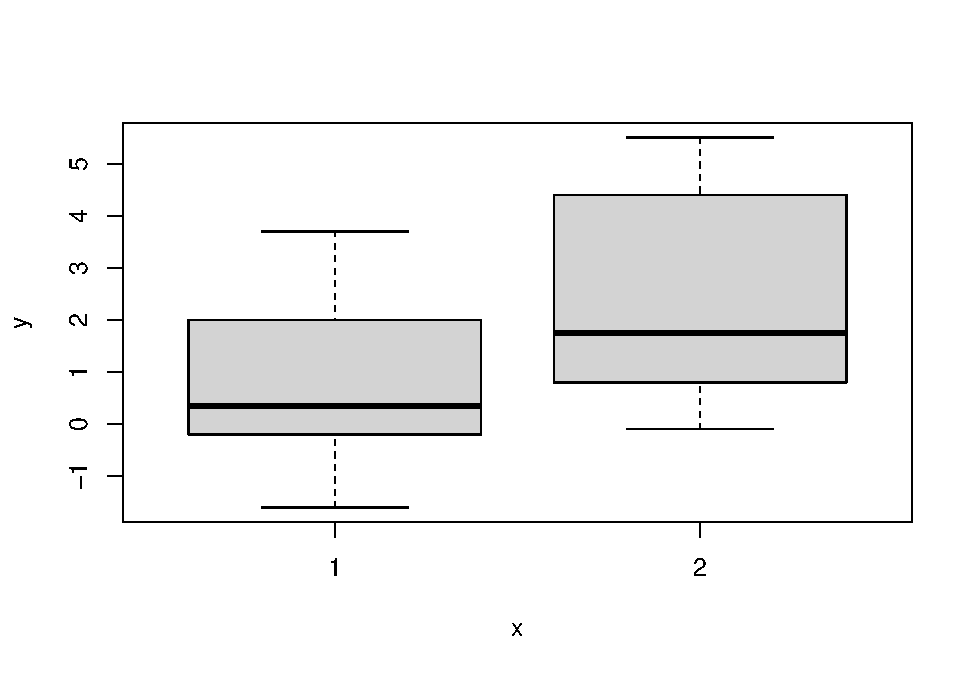
\includegraphics{gitbook-demo_files/figure-latex/unnamed-chunk-8-1.pdf}
\caption{\label{fig:unnamed-chunk-8}Generic Boxplot}
\end{figure}

The plot() function is an example of a generic function, which means it's a function that will try to adapt to our code. In this case, the plot() function looks at the variables we wants to plot, and identifies that the box plot is the most appropriate way to plot it.

Now this plot is perfectly adequate for a first viewing, but let's make it a bit more instructive by adding labels to the x and y axis, and by adding a title to it.

\begin{Shaded}
\begin{Highlighting}[]
\FunctionTok{plot}\NormalTok{(sleep}\SpecialCharTok{$}\NormalTok{group, sleep}\SpecialCharTok{$}\NormalTok{extra, }\AttributeTok{xlab =} \StringTok{"Treatment"}\NormalTok{, }\AttributeTok{ylab =} \StringTok{"Hours of Sleep"}\NormalTok{, }\AttributeTok{main =} \StringTok{"Effect of Treament on Sleep Duration"}\NormalTok{)  }
\end{Highlighting}
\end{Shaded}

\begin{figure}
\centering
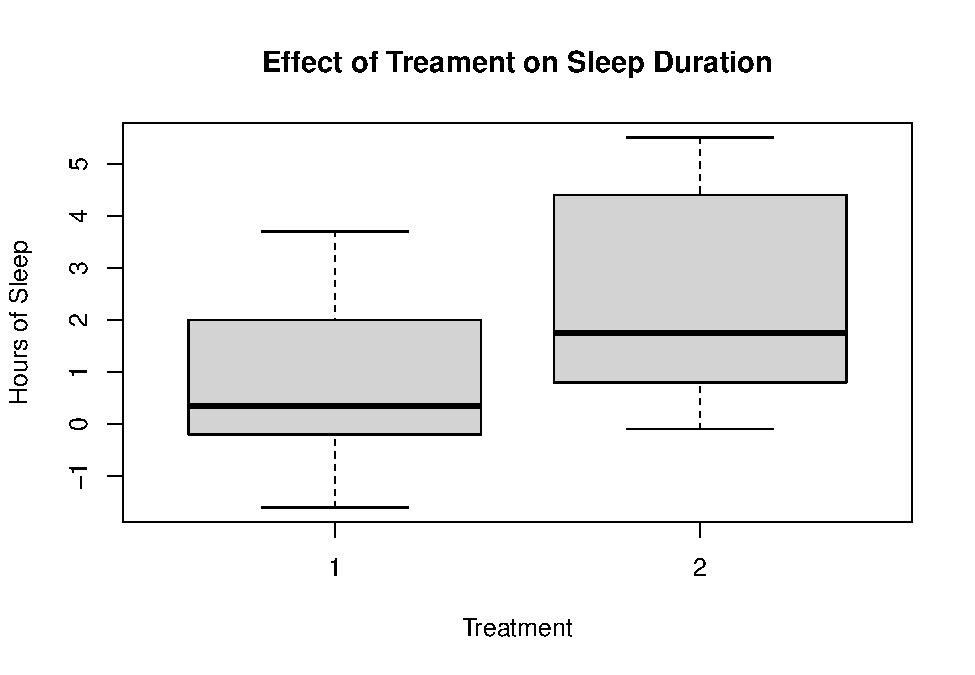
\includegraphics{gitbook-demo_files/figure-latex/unnamed-chunk-9-1.pdf}
\caption{\label{fig:unnamed-chunk-9}Generic Boxplot with appropriate labelling}
\end{figure}

\begin{Shaded}
\begin{Highlighting}[]
\CommentTok{\#xlab = creates a label for the x{-}axis  }

\CommentTok{\#ylab = creates a title for the y{-}axis  }

\CommentTok{\#main = creates a title for the plot  }
\end{Highlighting}
\end{Shaded}

Now let's take this plot and save it to a PDF so that we could share our results with others. The standard way of doing this in R is a bit cumbersome. We have to tell R that we are about to create a plot that we want to make into a PDF. Then we have to generate the plot. Then we have to tell R we are done with creating the PDF. We'll learn a MUCH simpler way to do this in future weeks, but this will do for now.

\begin{Shaded}
\begin{Highlighting}[]
\FunctionTok{pdf}\NormalTok{(}\AttributeTok{file =} \StringTok{"myplot.pdf"}\NormalTok{) }\CommentTok{\#Tells R that we will create a pdf file called "my\_plot" in our working directory}

\FunctionTok{plot}\NormalTok{(sleep}\SpecialCharTok{$}\NormalTok{group, sleep}\SpecialCharTok{$}\NormalTok{extra, }\AttributeTok{xlab =} \StringTok{"Treatment"}\NormalTok{, }\AttributeTok{ylab =} \StringTok{"Hours of Sleep"}\NormalTok{, }\AttributeTok{main =} \StringTok{"Effect of Treament on Sleep Duration"}\NormalTok{)  }\CommentTok{\#this will save the plot to our pdf}


\FunctionTok{dev.off}\NormalTok{() }\CommentTok{\#this tells R that we are done with adding stuff to our PDF}
\end{Highlighting}
\end{Shaded}

\begin{verbatim}
## pdf 
##   2
\end{verbatim}

Go to the files pane, and open up the pdf ``my\_plot1.pdf''. It should be in your working directory. Open it up the PDF and have a look at your graph\footnote{This is a fairly generic type of graph offered by base R. During the course we will looking at ways we can create ``sexier'' and more APA friendly type of graphs. But for one line of code, it's not bad!}.

There we have it! That completes our first session with R and RStudio. Today was more about getting to grips with the software R and RStudio, but we still got our first pieces of code written. Hopefully it's given you a tiny glimpse into what R can do.

Next week, we will go into more detail about programming concepts and how to import data.

\hypertarget{programming1}{%
\chapter{Basic R Programming (Part I)}\label{programming1}}

Today we are going to learn some basic programming concepts. By the end of the session, you should be able to:

\begin{itemize}
\item
  Run and troubleshoot commands in the R console.
\item
  Understand the different data types in R and how to create them.
\item
  Write comments to your code to better structure it.
\item
  Create and change variables.
\item
  Create and use functions.
\item
  Install R packages.
\item
  To use the help function in R.
\end{itemize}

\hypertarget{using-the-r-console}{%
\section{Using the R Console}\label{using-the-r-console}}

In the previous chapter, I made a distinction between the script and the console. I said that the script was an environment where we would write and run polished code, and the R console is an environment for writing and running ``dirty'' quick code to test ideas, or code that we would run one.

That distinction is kinda true, but it's not completely true. In reality, when we write a script we are writing \textbf{\emph{commands}} for R to \textbf{\emph{execute}} in the R console. When we ``run'' a script, we are feeding that script to the console. In this sense, the R script is equivalent to a waiter. We tell the waiter (R script) what we want to order, and then the waiter hands that order to the chef (R console).

So even though we will primarily not use the R console in this class, it's important to know how to work with it. We do not want the chef spitting in our food.

\hypertarget{typing-commands-in-the-console}{%
\subsection{Typing Commands in the Console}\label{typing-commands-in-the-console}}

The R console uses the operator ``\textgreater{}'' to indicate that it is ready for a new command. We enter in our code after this operator and press enter to compute it.

We can command the R console to compute calculations.

\begin{Shaded}
\begin{Highlighting}[]
\SpecialCharTok{\textgreater{}} \DecValTok{10} \SpecialCharTok{+} \DecValTok{20}

\NormalTok{[}\DecValTok{1}\NormalTok{] }\DecValTok{30}
\end{Highlighting}
\end{Shaded}

\begin{Shaded}
\begin{Highlighting}[]
\SpecialCharTok{\textgreater{}} \DecValTok{20} \SpecialCharTok{/} \DecValTok{10}

\NormalTok{[}\DecValTok{1}\NormalTok{] }\DecValTok{2}
\end{Highlighting}
\end{Shaded}

If you are performing calculations in R, it's important to know that it follows the usual arithmetic convention of order of operations (remember \href{https://www.tes.com/en-ie/teaching-resource/bidmas-bodmas-bedmas-bimdas-pemdas-permdas-11154272\#:~:text=\%E2\%80\%A2\%20BIMDAS\%20\%2D\%20Brackets\%2C\%20Indices\%2C,Multiplication\%2C\%20Division\%2C\%20Addition\%2C\%20Subtraction}{BIMDAS - Bracets, Indices, Multiplication, Division, Addition, and Subtraction?}).

\begin{Shaded}
\begin{Highlighting}[]
\SpecialCharTok{\textgreater{}}\NormalTok{ (}\DecValTok{20} \SpecialCharTok{+} \DecValTok{10} \SpecialCharTok{/} \DecValTok{10}\NormalTok{) }\SpecialCharTok{*} \DecValTok{4} 

\NormalTok{[}\DecValTok{1}\NormalTok{] }\DecValTok{84}

\SpecialCharTok{\textgreater{}}\NormalTok{ ((}\DecValTok{20} \SpecialCharTok{+} \DecValTok{10}\NormalTok{) }\SpecialCharTok{/} \DecValTok{10}\NormalTok{) }\SpecialCharTok{*} \DecValTok{4}

\NormalTok{[}\DecValTok{1}\NormalTok{] }\DecValTok{12}
\end{Highlighting}
\end{Shaded}

Now you'll have noticed that the output of every line of code we entered starts with a {[}1{]} before our actual result. What does this mean?

Think of the square brackets with a number as a way for R to label and organize its responses. Imagine you have a conversation with R, and every time you ask it something, it gives you an answer. The square brackets with a number, like \textbf{\texttt{{[}1{]}}}, are like labels on each response, telling you which answer corresponds to which question. This is R \textbf{\emph{indexing}} its answer.

In each of the above examples, we asked R one question \textbf{\emph{per each}} command, which is why the answer is always {[}1{]}. If we entered longer code with multiple questions, then we could multiple answers. We could tell which answer related to which question through the index. This is really useful when we ask R long and more complicated questions.

  \bibliography{book.bib,packages.bib}

\end{document}
